%\documentclass[a4paper,10pt]{article}
\documentclass[letterpaper, 12pt, conference]{ieeeconf}
\usepackage{amsmath} % For 'cases' curly brace
\usepackage{amsfonts} % For bold number set font
\usepackage{color}
\usepackage{algorithmic}
\usepackage{algorithm}
\usepackage{amssymb}
\usepackage{array}
\usepackage{url}
\usepackage{graphicx}
\usepackage{subcaption}

\usepackage[font=bf]{caption}

\newcommand{\xxx}[1]{\textcolor{red}{#1}}

\begin{document}
\title{\LARGE \bf
Validating Cell Tower Clustering for Mobility Prediction
}
\author{Mehrdad Moradi\\moradi@umich.edu \and Pedro d'Aquino\\
pdaquino@umich.edu}
\date{December 11, 2012}

\maketitle

\begin{abstract}
We investigate in detail one of the algorithms involved in cellular mobility 
prediction. These systems try to predict a user's position based on cell 
tower connections. One key difficulty in this is the oscillation effect: a 
stationary phone will often switch between towers, adding significant noise 
to the data. We look at the efficiency of one of the approaches in the 
literature that tries to counter this effect.  This algorithm tries to 
cluster cell towers that users often oscillate between. In order to do 
evaluate the algorithm's efficiency, we use a new dataset that allows us to 
infer GPS data for cell towers. We find that the algorithm performs well.
\end{abstract}
\xxx{Make sure I didnt write Mobility Data Challenge (it should be Mobile 
data challenge), or OpenCell (it should be open dataset).}

\section{Introduction}
\label{sec:intro}

In this project, we address one of the challenges faced in mobility 
prediction using GSM cell tower connection logs. In our context, mobility 
prediction in cellular
towers can be defined as the ability to predict a user's physical movement by 
examining the history of cell tower connections. This is very important
for mobile network operators, as several network optimizations are possible 
if they can forecast with reasonable accuracy
where a user will be in the future \cite{LeapGraph} \cite{Liu97anoptimal}. By 
being able to pre-allocate resources to towers that are most likely to
be connected to by the user, network operators can improve latency and 
uptime. This is increasingly important as the amount of data in cellular 
networks
increases: indeed, in 2010 the amount of data traffic surpassed voice traffic 
for the first time, and it is expected to double annually in the near future
\cite{EricssonData}.

Another use of mobility prediction is to discover mobility profiles, i.e. 
patterns in a user's movement \cite{mobilityprofiler}. As illustrated in \cite
{mobilityprofiler}, mobility profiles have a wide range of possible 
applications, from traffic planning to advertisement. Recently, Google 
started integrating
a contextual search and recommendation service in its phones that is able to, 
for instance, detect a user's home and work addresses and suggest routes 
based on
traffic \cite{googleNow}.


The heart of every mobility prediction system based on cell tower connections 
is to infer movement based on which cell the user's phone is connected to. 
The goal
is to predict which tower the user is more likely to connect to next. A major 
challenge in this is dealing with the \textit{oscillation effect}, which 
happens when a \textit{stationary} user's phone switches between two or more 
towers. Figure~\ref{fig:stationary} shows an example of a stationary phone 
that connects to different cell towers. This is a natural consequence of the 
radio medium and the fact that towers very often have overlapping ranges. In 
order to accurately predict a user's mobility, these outliers have to be 
removed so that fluctuations can be separated from actual user movement.

In this project, we analyze one published algorithm for oscillation detection 
\cite{mobilityprofiler} and evaluate its performance using GPS data as ground-
truth. We find that this algorithm performs surprisingly well as measured by 
two metrics we define.

This report is structured as follows. In the next section, we motivate our 
work by explaining why clustering validation is important.
In section~\ref{sec:methodology} we describe our methodology  and explain the algorithm we 
will evaluate. We present and discuss results in section~\ref{sec:results}, 
and conclude in section~\ref{sec:conclusion}.

\begin{figure}
\centering
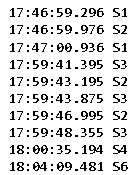
\includegraphics[width=0.15\textwidth]{figs/stationary_oscillation}
\caption{An example of actual cell tower connection logs for a stationary 
phone, slightly modified from~\cite{LeapGraph}. The time of the sample is on 
the left, and an identifier for the cell tower is on the right. We can see 
that the phone connects to several towers, even though it does not move. }
\label{fig:stationary}
\end{figure}

\section{Motivation}

The accuracy of current mobility prediction systems based on cell tower 
connections is usually measured through machine learning techniques like cross
-validation that try to validate the ultimate goal of forecasting the user's 
future connections \cite{LeapGraph}. As far as we know there are no studies 
that evaluate methods of dealing with the oscillation effect, even though all 
prediction systems must deal with it.

In this paper we report the results of such an analysis. We have implemented 
and evaluated the ``oscillation graph'' technique described in \cite{
mobilityprofiler}. The basic idea of this algorithm is to detect cell towers 
that often present oscillations and consider them as a single tower. This is 
effectively a clustering algorithm. Our goal is to evaluate whether towers 
that are clustered together are actually close in real life. To evaluate 
this, we use the Nokia Mobility Challenge dataset, which has data on both 
cell tower connection (``GSM logs'') and the GPS position of the phones.

\section{Methodology}
\label{sec:methodology}

The Mobility Profiler paper \cite{mobilityprofiler} describes an algorithm to 
detect the oscillation effect. Our approach to evaluating this algorithm's 
efficiency was the following. We implement the algorithm as described in \cite
{mobilityprofiler} and test it in the same dataset used in the original 
paper. However, that dataset does not have any data on the location of the 
users when they were connected to the towers. We therefore apply the 
algorithm to another dataset, from the Nokia Mobility Challenge, in which the 
GPS position of the users is listed. In order to evaluate how successful the 
clustering algorithm is, we devise two metrics: cluster distance and cluster 
incompleteness.

\subsection{Clustering algorithm}

There are two main papers that tackle the problem of oscillation effects: the 
Mobility Profiler paper, by Bayir et al. \cite{mobilityprofiler}, and the 
Leap Graph paper by Duffield et al \cite{LeapGraph}. Ideally we would want to 
evaluate both of them, but the leap graph algorithm, which was published by 
researchers at AT\&T, makes use of the active set of connections. The active 
set contains all towers that are within range of the phone's antenna at any 
given time. Unfortunately, active set logs are not public which makes it 
impossible for us to evaluate the leap graph algorithm.

We therefore focus our efforts on the algorithm described in the Mobility 
Profiler paper, which we call the oscillation graph algorithm. In the 
interest of completeness, we briefly describe how it works.

\begin{figure*}
        \centering
        \begin{subfigure}[t]{0.44\textwidth}
                \centering
                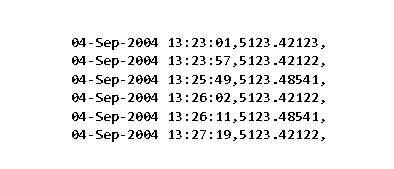
\includegraphics[width=\textwidth]{figs/gsm_log_rm}
                \caption{A series of timestamped GSM cell tower connection 
log records, from the Reality Mining dataset. The cell tower is identified by 
an area code and a cell ID, which are separated by a period. In this 
particular example it seems that all three towers are oscillating.}
                \label{fig:gsm_log_example}
        \end{subfigure}%
        \qquad %add desired spacing between images, e. g. ~, \quad, \qquad etc. 
          %(or a blank line to force the subfigure onto a new line)
        \begin{subfigure}[t]{0.48\textwidth}
                \centering
                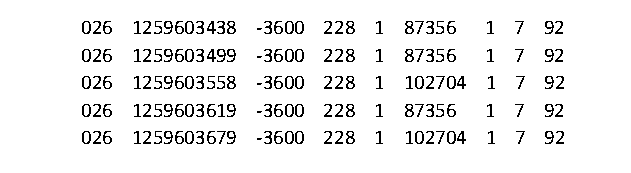
\includegraphics[width=\textwidth]{figs/gsm_log_mdc}
                \caption{An example of GSM records in the Nokia Mobile Data 
Challenge. From left to right, the fields are: user id, timestamp, time zone, 
country ID, network ID, cell ID, area ID, signal strength from 1 to 7 and 
signal strength in dBm.}
			\label{fig:gsm_log_mdc}
        \end{subfigure}
				\caption{Example of GSM cell tower connection logs in both datasets 
we use.}
\end{figure*}

\subsubsection{Mobility paths}
The input of the algorithm is a sequence of \textit{handovers}, which are 
transition events when a phone switches the tower it is connected to. These 
events are timestamped, as shown in Figure~\ref{fig:gsm_log_example}. The 
first step of the algorithm is to analyze the transitions and extract \textit{
mobility paths}.  A mobility path corresponds to a sequence of handovers that 
are associated with actual user movement. For example, imagine a user that 
drives every morning to work, stays there for eight hours and goes back home. 
During his drive to work, the user's phone will switch cell towers several 
times. These handovers will be included in a mobility path. While the user is 
at work, ignoring the oscillation effect temporarily, the phone will be 
connected to a single tower. Finally, when the user the goes home the 
handovers that occur during the drive will belong to a different mobility path.

More formally, let $\Delta_i$ be the time difference between two consecutive 
handovers for a particular user's connection log. In other words, $\Delta_i$ 
is the time the user spent connected to cell tower $C_i$. Let $\delta_{
duration}$ be the \textit{end-location threshold}. Then we define a mobility 
path as a sequence of cell connections $\left\{C_i, C_{i+1}, \ldots, C_j
\right\}$ such that $\Delta_i < \delta_{duration}$ for all handovers.\footnote
{We also have to consider \textit{hidden end-locations}, which happen when a 
user's phone is disconnected from any towers, or if the user turns his phone 
off. We omit its formal definition for briefness.}


\subsubsection{Oscillating pair detection}

The goal of the oscillation detection algorithm is to retrieve sets of towers 
that overlap each other -- that is, towers that could be in a stationary 
user's handover logs. The main idea behind the algorithm is that a user's 
phone is more likely to switch between oscillating towers than between 
regular towers that are not overlapping. In this context, \textit{switching} 
means a handover from one tower to another inside of a mobility path. We can 
define $\delta_{osc}$ to be the minimum switching count and consider all 
pairs of towers that have more than $\delta_{osc}$ switches in one mobility 
path to be an \textit{oscillating pair}. The example in \cite{mobilityprofiler}
is illustrative: consider a sequence of handovers $\left[x, y, x, w, v, w, y
\right]$ where every element represents one cell tower. We say that the pair $
(x, y)$ has 3 switches: the first two from $x$ to $y$ and back to $x$ in the 
first positions of the sequence, and then back to $y$ at the end. Hence, if 
we adopt $\delta_{osc}=3$ the only oscillating pair would be $(x, y)$. Note 
that switches do not need to be consecutive. The authors argue that this 
allows for detection of overlapping towers in dense region where multiple 
towers may be within range at the same time.

\subsubsection{Oscillation graph}

After detecting all the oscillating pairs in all mobility paths, the next 
step is to build the oscillation graph. The set $V$ of vertices in the graph 
are all cell towers in the dataset, and the weighted edges in $E$ connect 
oscillating pairs. Let $P_i$ be a mobility path.The weight of every edge, 
which we also call its \textit{support}, is defined as:

\begin{equation*}
s(x,y) = \frac{|\left\{P_i| (x, y) \in P_i \wedge (x, y) \text{oscillated}
\right\}|}{|\left\{P_i| (x, y) \in P_i\right\}|}
\end{equation*}

In words, $s(x,y)$ is the ratio of how many times the cell towers $x$ and $y$ 
oscillated over the number of mobility paths in which $x$ and $y$ appear. For 
example, a pair of towers such that in \textit{every} mobility path that both 
of them appear the switch count is greater than $k$ would have a support 
equal to 1. If a pair only switches more or equal to $k$ times in half the 
mobility paths both of the towers appear in, that pair's support would be 0.5.

\subsubsection{Oscillation graph clustering}

The final step of the algorithm is to find clusters in the oscillation graph. 
Intuitively, a cluster represents a group of towers that are not indicative 
of actual user movement. The Mobility Profiler paper uses an greedy divise 
algorithm for clustering. At every iteration, the algorithm removes the edge 
with the lowest weight from the graph. It then evaluates the ``quality'' of 
all connected components, which is the weighted ratio of edges inside of the 
cluster over the number of edges that leave the cluster in the original 
graph. Formally, let $C$ be a cluster with the set of edges $E$, and $E_{out}$
 be the set of edges that have exactly one vertex in $C$, and define $w(e)$ 
to be an edge's weight:

\begin{equation*}
Q(C) = \frac{\displaystyle\sum_{\forall e_{in} \in E}{w(e_{in})}}{
\displaystyle\sum_{\forall e_{out} \in E_{out}}{w(e_{out})}}
\end{equation*}

Every cluster with quality metric greater than a threshold is removed from 
the graph. The algorithm continues until there are no more vertices in the 
graph. The algorithm outputs all the clusters it found. Our main goal is to 
evaluate these clusters according to the GPS position of the users when they 
were within range of that tower.



\subsection{GSM datasets}

We use two datasets with GSM cell tower connection data, from the Reality 
Mining project and from the Nokia Mobile Data Challenge.

\subsubsection{Reality Mining}

The Reality Mining dataset (RM)~\cite{rm} was obtained from over 330 thousand 
hours of data logged from 94 volunteers' cell phones during 2004. The breadth 
of information collected is impressive, ranging from cell tower IDs to which 
Bluetooth devices are within 5 meters of the users. This dataset has been 
widely used in research into social and friendship networks. For our project, 
following~\cite{mobilityprofiler}, the focus is the cell tower connection logs.

\subsubsection{Nokia Mobile Data Challenge -- GSM}

The Nokia Mobile Data Challenge (MDC) project~\cite{nokiaMdc} gathered data 
from 170 volunteers in the Swiss city of Lausanne during 2009. In comparison 
to the Reality Mining project, more sensors were available for the 
researchers (a consequence of the evolution of mobile phones) and the 
population was more diverse (two thirds of the volunteers were employed). In 
particular, there is data available on the users' cell tower connections, 
which is essential for mobility prediction. However, while the Reality Mining 
dataset logs every cell transition, the MDC authors sample the active cell 
tower connection every minute. This leads to some data loss, since cell 
transitions can happen at a much higher frequency (e.g.
Figure~\ref{fig:gsm_log_example}). An example of the GSM logs in the MDC is shown in
Figure~\ref{fig:gsm_log_mdc}.

\subsection{Cell location datasets}

Our main contribution is an analysis of the oscillation clustering algorithm 
using GPS data. We use two sources of GPS data, the Nokia MDC and the 
OpenCell database.

\subsubsection{Nokia Mobility Data Challenge -- GPS}

Phones in the MDC also had their GPS units sampled every minute, recording 
the latitude and longitude of the user's phone. We process the GPS and try to 
establish an approximate position for each cell tower. We approximate the 
cell tower position as the average of the positions of users when they were 
connected to that tower. To do this, we have to match each entry in the GSM 
log with an entry in the GPS log.

Because GSM and GPS entries do not necessarily have the same timestamp (in 
fact, they almost never do), we use GPS entries that have a timestamp within $
\delta_{GPS}$ seconds of the GSM entry we are trying to match. The algorithm 
goes through every record in the GSM log and tries to find a matching GPS 
log. After going through all users' connection logs, we estimate each tower's 
position as the average of all GPS positions that were associated with that 
tower. It is important to have a measure of how accurate the GPS estimate of 
a particular tower is, so we record the number of GPS samples for that tower 
and the standard deviation in the samples. The standard deviation is computed 
based on the distance from each sample to the average point, which is 
calculated using the Haversine formula \cite{haversine}. In the experiments in this
report we used $\delta_{GPS}=40$~seconds.

The algorithm runs in $O(k(n\log n + m\log n))$, where $k$ is the number of 
users in the dataset and $m$ and $n$ are upper bounds on the number of GPS 
and GSM records per user, respectively. The logarithmic factor comes from 
sorting the GPS log by timestamp and performing a binary search.

\subsubsection{OpenCellId and OpenBMap (open dataset)}

OpenCellID~\cite{openCellId} and OpenBmap~\cite{openBMap} are two open source 
projects with the goal of providing researchers with a complete database of 
cells towers and their locations They gather the data through users who 
voluntarily participate in the project by adding a logging component to their 
phones that keeps track of the position and associates it with a cell tower. 
OpenBMap has over 791694 cells in its database, while OpenCellID covers 
1889463. In our application we combine both measures and use an average, 
which we refert to as the ``open dataset''.

\section{Results}
\label{sec:results}

\begin{table*}
    \centering
    \begin{tabular}{ | c || r | r | r | r | r | }
    \hline
    Dataset & Cells  & Area codes & Country IDs & Handovers & Clusters \\
    \hline
    Nokia Mobile Data Challenge & 23378 & 966 & 33 & 3308612 & 869 \\
    \hline
    Reality Mining & 32787 & 32787 & 2 & 32787 & 32787 \\
    \hline
    \end{tabular}
\caption{Comparison between the Nokia Mobile Data and Reality Mining datasets.}
\label{tbl:datasetComparison}
\end{table*}


We implemented the clustering algorithm in \cite{mobilityprofiler} for the 
Reality Mining and the Nokia Mobility Data Challenge datasets and compared 
the results of the clustering in both datasets (adjusting for the fact that 
the MDC dataset's data is sampled every minute). In this section, we report 
the results of running the algorithm in those datasets and analyze the 
results. We find that the Reality Mining and MDC datasets have similar 
patterns of cluster size and density. We also used GPS data to evaluate the 
accuracy and quality of the resulting clusters. Our experiments show that the 
clustering algorithm performs well on both metrics we define.

Running the clustering algorithm on the RM dataset was more challenging than 
originally expected; there were inconsistencies with the dates (apparently 
the phones' clocks reverted to 01/01/2004 when the battery died) and time (
with entries appearing in an inconsistent order. We dealt with these problems 
by ignoring records with a timestamp equal to 01/01/2004 and by assuming that 
the ordering of the lines in the dataset logs represented the actual ordering 
that the logs were collected -- this seemed consistent with manual analysis 
of the logs and generated valid mobility paths\footnote{A valid mobility path 
is one in which there is no overlap of handovers -- that is, there cannot be 
two cells connected at the same time.}, which is not the case if the 
timestamps are taken at face value.

In all experiments we used the same parameters value as the original Mobility 
Profiler paper, namely $\delta_{duration} = 10 \text{minutes}$ and $\delta_{
osc} = 3$.

\subsection{Dataset comparison}

\begin{figure}
\centering
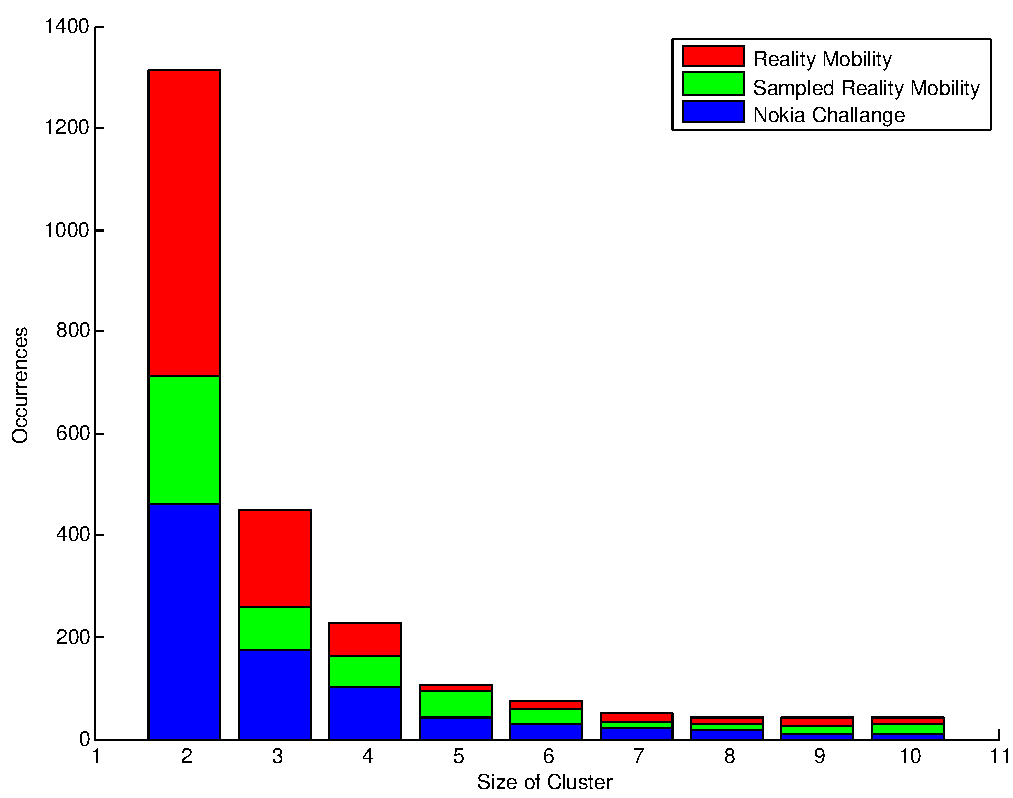
\includegraphics[width=0.48\textwidth]{figs/cluster_size}
\caption{The histogram of the size of clusters in the Reality Mining and 
Nokia Mobile Data Challenge datasets. Because the MDC dataset originates from 
sampling the user's phone every minute, we also sample the RM data to 
visualize the impact of sampling. We see that both datasets produce clusters 
that follow a similar size distribution.}
\label{fig:cluster_size}
\end{figure}

\begin{figure}
\centering
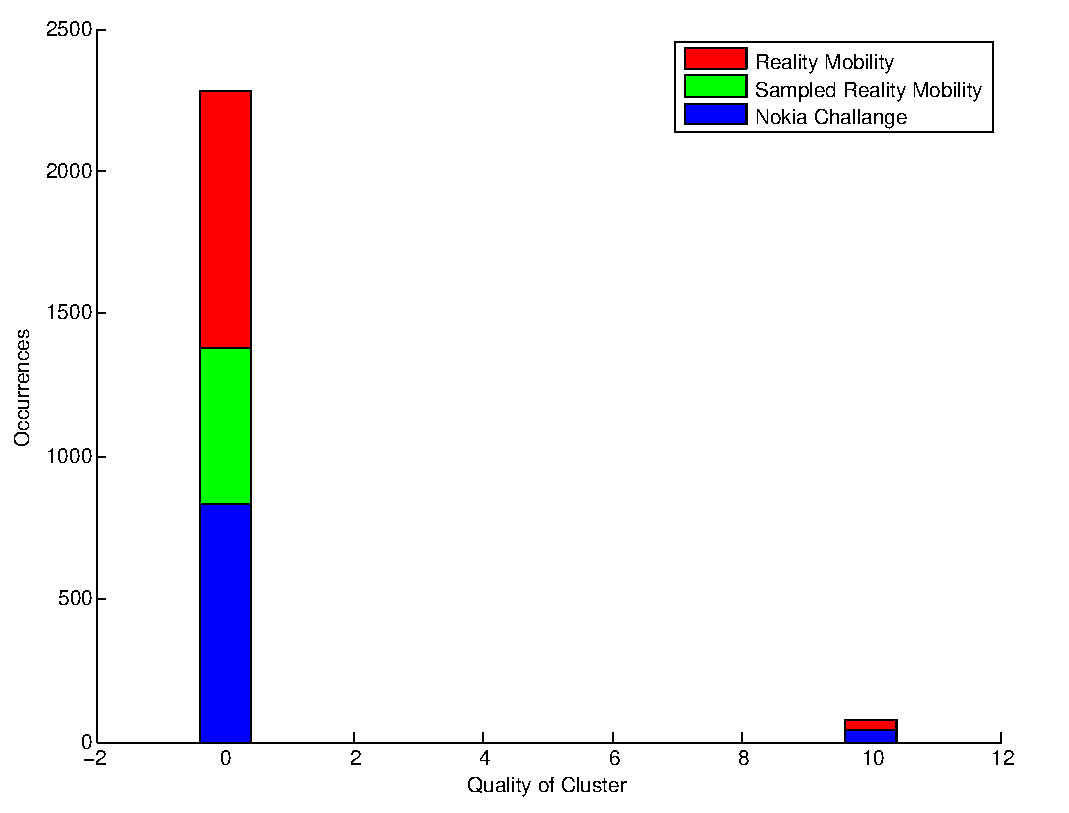
\includegraphics[width=0.48\textwidth]{figs/cluster_quality}
\caption{The histogram of the value of the quality metric for clusters in the 
Reality Mining and Nokia Mobile Data Challenge datasets. Clusters that have a 
quality metric of infinity are shown here as 0. We see that both datasets 
produce clusters that follow a similar size distribution.}
\label{fig:cluster_quality}
\end{figure}

\begin{figure}
\centering
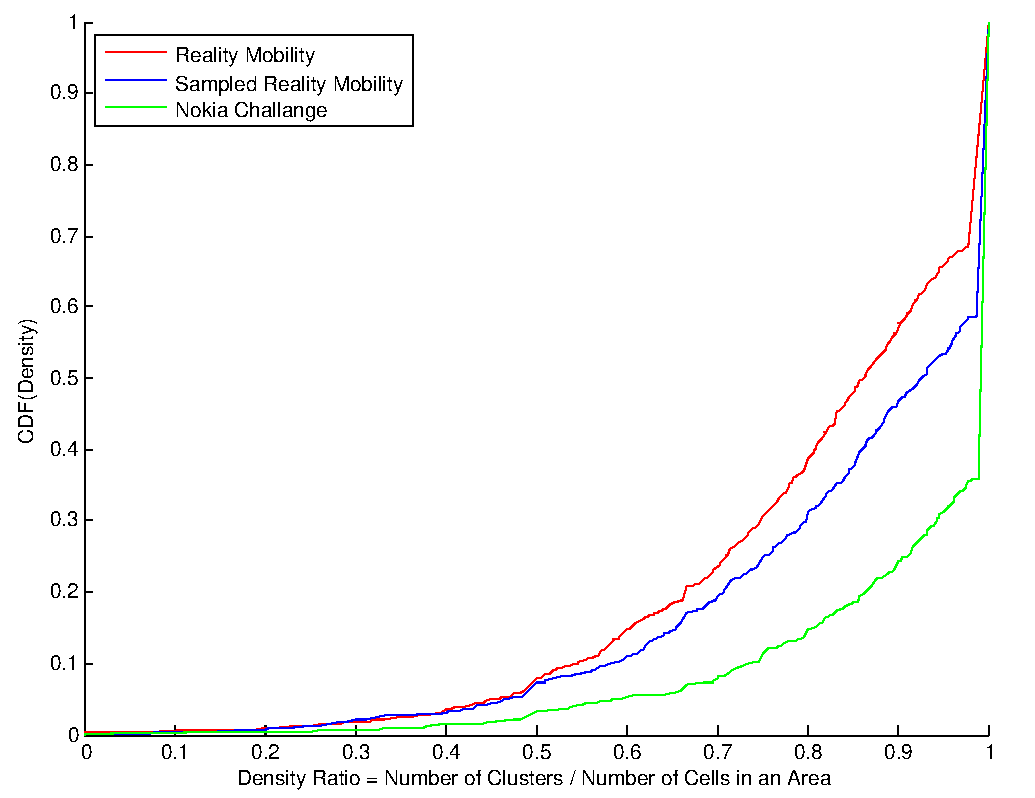
\includegraphics[width=0.48\textwidth]{figs/cluster_area_density}
\caption{The cummulative distribution function of the density of clusters in 
an area code. We define the density as the number of clusters over the number 
of cells in an area. An area with few, large clusters would have a density 
close to zero, while an area with very few clusters will have a density close 
to 1.}
\label{fig:cluster_area_density}
\end{figure}

\begin{table}
    \centering
    \begin{tabular}{ | m{2.8cm} || r | m{3cm} | }
    \hline
    Criteria & Cells & Fraction of all cells in MDC dataset \\
    \hline
		With GPS data & 7508 & 31.75\%  \\
    \hline
		More than one GPS sample & 5622 & 23.78\% \\
    \hline
		More than five  GPS samples & 3644 & 15.41\% \\
    \hline
		GPS samples with  std. deviation~$ < 500$\,m & 3024 & 12.79\% \\
    \hline
		GPS samples with  std. deviation~$ < 150$\,m & 1173 & 4.96\% \\
    \hline
    \end{tabular}
\caption{Statistics about the GPS data from the MDC GPS logs, for different 
levels of data ``reliability''. In most of the paper we only consider the 
location of a cell known when the GPS samples of that cell have standard 
deviation less than 500\,m. }
\label{tbl:gsm_logs_stats}
\end{table}

We compare the Reality Mining dataset, which was originally used in the 
Mobility Profiler paper, with the Mobility Data Challenge.
Table~\ref{tbl:datasetComparison} shows the number of cells, area codes and countries 
that are represented in each dataset. We can see that the MDC data has a much 
larger breadth in terms of the country IDs that are covered\footnote{We do 
not know the reason for this, since the researchers claim the data was 
collected entirely in Lausanne. It is possible that the volunteers simply 
travelled to many countries.}, but contains less cells and cell transitions.

However, both datasets show similar patterns in cluster size distribution, as 
evidenced in Figure~\ref{fig:cluster_size}, which also presents the cluster 
size distribution for the Reality Mining dataset sampled every minute. This 
is necessary for a fair comparison since the RM contains information on every 
handover, while the MDC samples the tower the phone is currently connected to 
every minute (so there is loss of information).

We have also evaluated the cluster quality metric in both datasets, and 
present the results in Figure~\ref{fig:cluster_quality}. Clusters whose cells 
have no outgoing edges in the original oscillation graph have a quality 
metric of infinity; these are represented as 0 in the histogram\footnote{This 
is an unfortunate consequence of the quality metric adopted by the Mobility 
Profiler paper. In section~\ref{sec:conclusion} we suggest an alternate 
metric that is always between 0 and 1.}. We see that this is the case for the 
vast majority of cells in both datasets.

Finally, we also compare the density of clusters with respect to area codes 
in Figure~\ref{fig:cluster_area_density}. We can also see that all datasets 
follow similar patterns.

The fact that both datasets show a similar distribution is important for our 
results, since it allows us to extrapolate the results we find with the MDC 
dataset to the RM dataset with reasonable confidence.

\subsection{Location statistics}
\label{sec:location_stats}
Table~\ref{tbl:gsm_logs_stats} shows some statistics about the GPS 
information obtained from the GPS logs in the MDC dataset. We use two 
criteria to judge the confidence we have in a particular cell's position 
estimate: the number of GPS samples for that cell and their standard 
deviation. In the clustering efficiency analysis of
Section~\ref{sec:effectiveness} we only consider cells that have more than one GPS sample 
and whose samples' standard deviation is less than 500\,m. We choose these 
parameters as they offer a good tradeoff between precision and sample size (
for instance, choosing a stricter criteria of $\sigma < 150$ would leave us 
with less than 5\% of all cells).

\begin{figure}
\centering
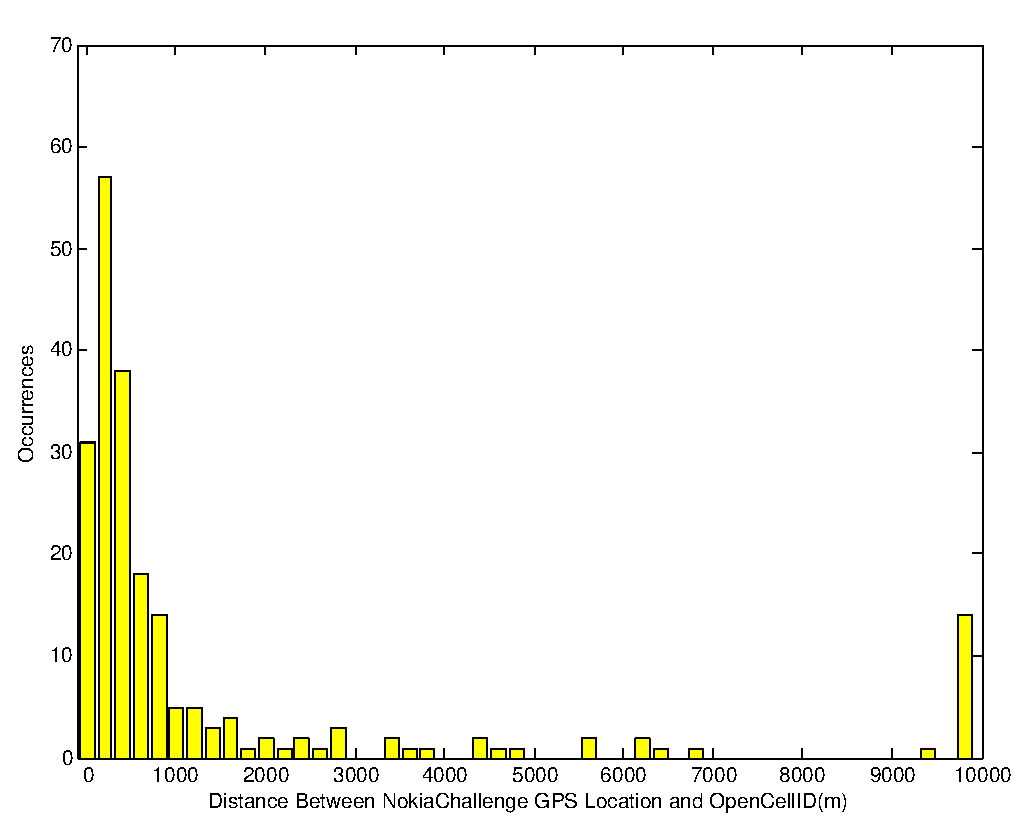
\includegraphics[width=0.48\textwidth]{figs/mdc_open_distance}
\caption{The histogram of the distance between cell tower positions estimated 
using the GPS logs from the MDC dataset and the position in the open datasets.}
\label{fig:mdc_open_distance}
\end{figure}

The data from the open dataset covers 5859 cells in the MDC dataset, or 24.78
\%. We cannot use the data on the Reality Mining dataset, because the network 
ID is not specified in its logs. Figure~\ref{fig:mdc_open_distance} shows a 
histogram of the distance between the position of cell towers as computed by 
MDC GPS logs and the open dataset. We see that the distance is usually small, 
which reinfornces our confidence in the MDC GPS logs. We analyze how many 
cells are covered by the combination of the open dataset and the GPS logs 
from the MDC in Table~\ref{tbl:open_mdc_stats}. It is clear that a strikingly 
small number of cells are present in both the MDC GPS logs and the open 
dataset -- and the fraction becomes almost insignifcant when we restrict the 
analysis to reliable GPS positions (those with small standard deviation in 
the samples).
\begin{table}
    \centering
    \begin{tabular}{ | m{2.8cm} || r | m{3cm} | }
    \hline
    Criteria & Cells & Fraction of all cells in MDC dataset \\
    \hline
		With GPS data from MDC and open datasets & 1645 & 6.96\%  \\
    \hline
		More than one GPS sample in MDC & 1220 & 5.16\% \\
    \hline
		More than five  GPS samples in MDC & 680 & 2.88\% \\
    \hline
		GPS samples in MDC with  std. deviation~$ < 500$\,m & 593 & 2.51\% \\
    \hline
		GPS samples in MDC with  std. deviation~$ < 150$\,m & 216 & 0.91\% \\
    \hline
    \end{tabular}
\caption{Statistics for cells for which we have GPS data from the MDC GPS 
logs \textit{and} the open datasets. We see that very few cells have a 
reliable set of GPS samples in the MDC database and are present in the open 
dataset. }
\label{tbl:open_mdc_stats}
\end{table}


\begin{figure*}
        \centering
        \begin{subfigure}[t]{0.48\textwidth}
                \centering
                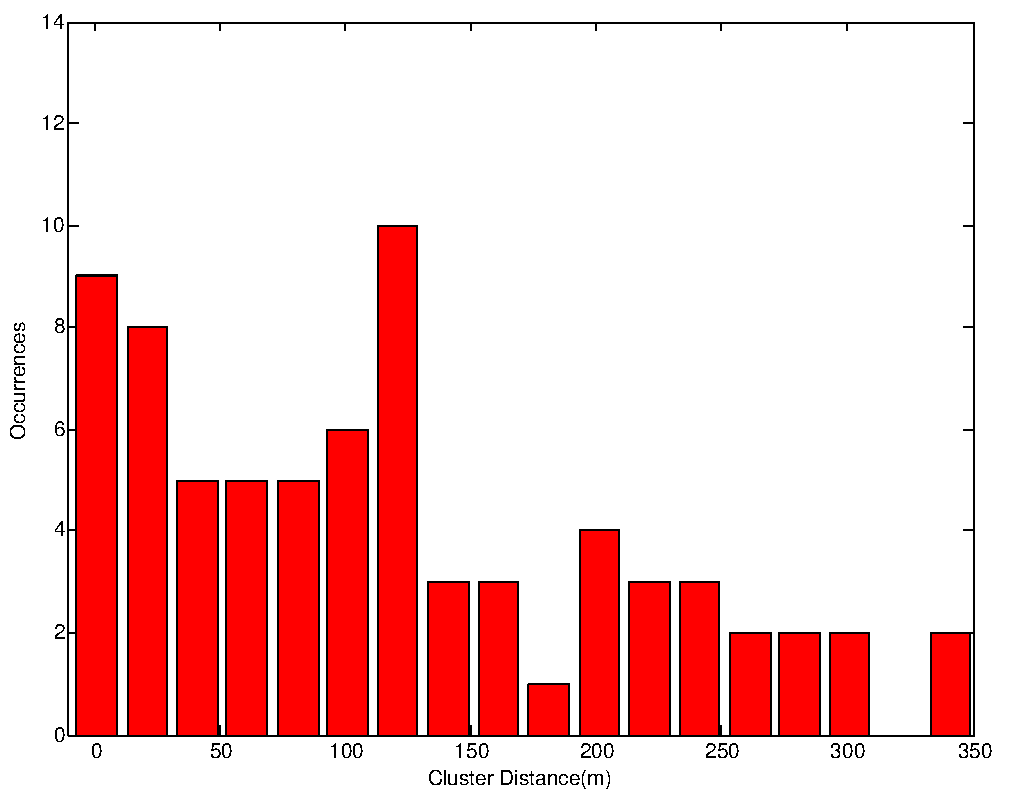
\includegraphics[width=\textwidth]{figs/cluster_distance_hist}
                \caption{The histogram of the cluster distance for the MDC 
dataset, using GPS data with $\sigma < 500$ from the MDC dataset. We only 
consider clusters for which we have GPS for more than 70\% of the cells. We 
observe that few clusters have a significant cluster distance.}
                \label{fig:cluster_distance_hist}
        \end{subfigure}%
        ~ %add desired spacing between images, e. g. ~, \quad, \qquad etc. 
          %(or a blank line to force the subfigure onto a new line)
        \begin{subfigure}[t]{0.48\textwidth}
                \centering
                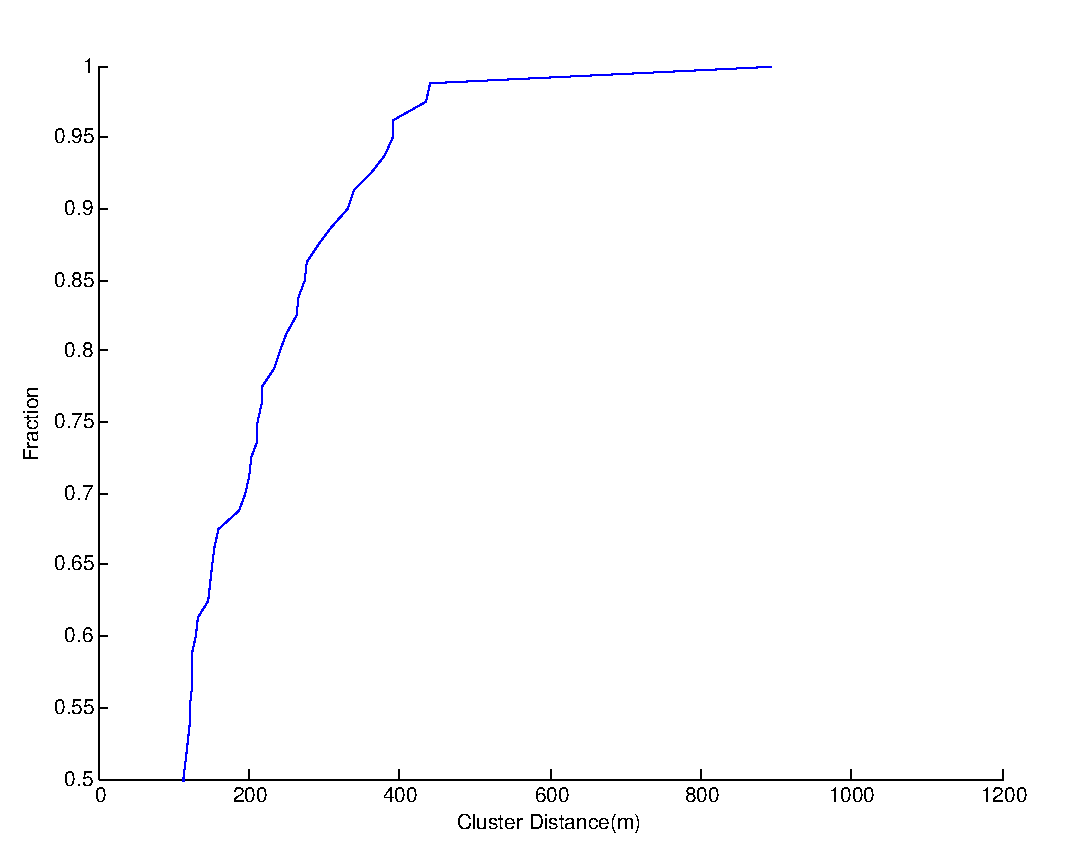
\includegraphics[width=\textwidth]{figs/cluster_distance_cdf}
                \caption{The CDF of the cluster distance under the same 
conditions. Nearly all clusters have a distance metric less than 500\,m.}
                \label{fig:cluster_distance_cdf}
        \end{subfigure}
				\caption{Cluster distance measurements.}\label{fig:cluster_distance}
\end{figure*}

\begin{figure*}
        \centering
        \begin{subfigure}[t]{0.48\textwidth}
                \centering
                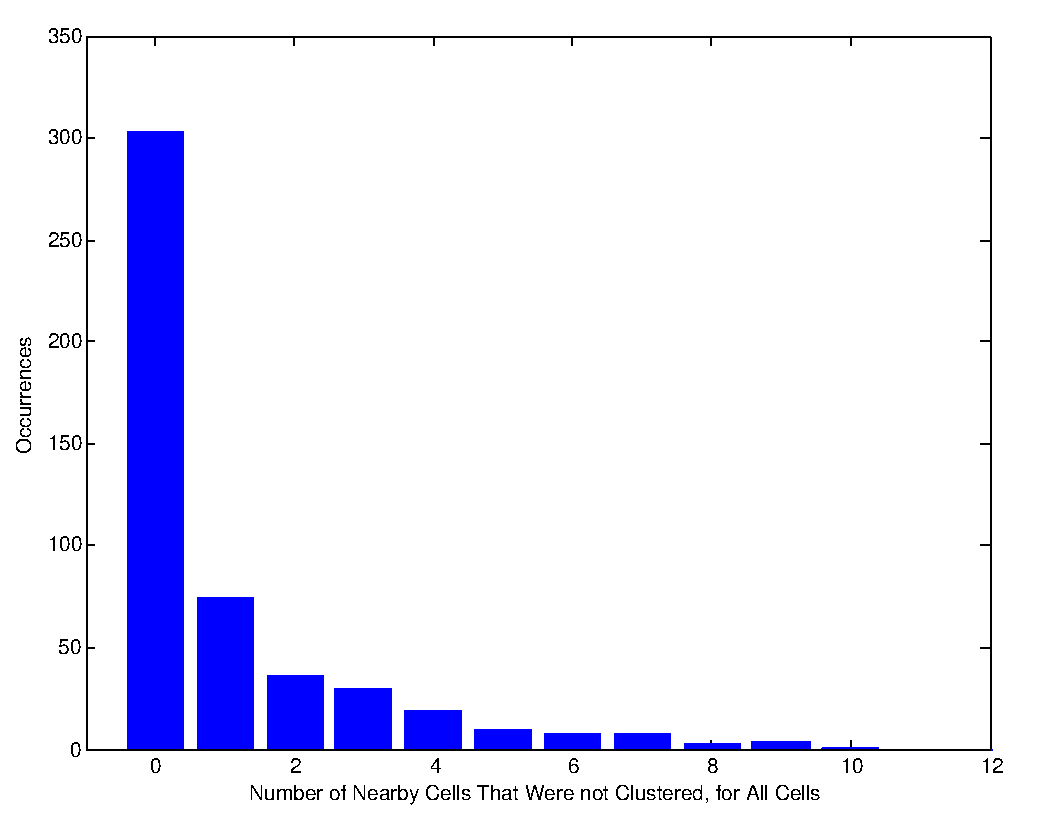
\includegraphics[width=\textwidth]{figs/cluster_incomp_hist}
                \caption{The histogram of the cluster incompleteness for the 
MDC dataset, using GPS data with $\sigma < 500$ from the MDC dataset. A large 
number of cells have an incompleteness measure of 0, which means all nearby 
cells were clustered (or there weren't any nearby cells).}
                \label{fig:cluster_incomp_hist}
        \end{subfigure}%
        ~ %add desired spacing between images, e. g. ~, \quad, \qquad etc. 
          %(or a blank line to force the subfigure onto a new line)
        \begin{subfigure}[t]{0.48\textwidth}
                \centering
                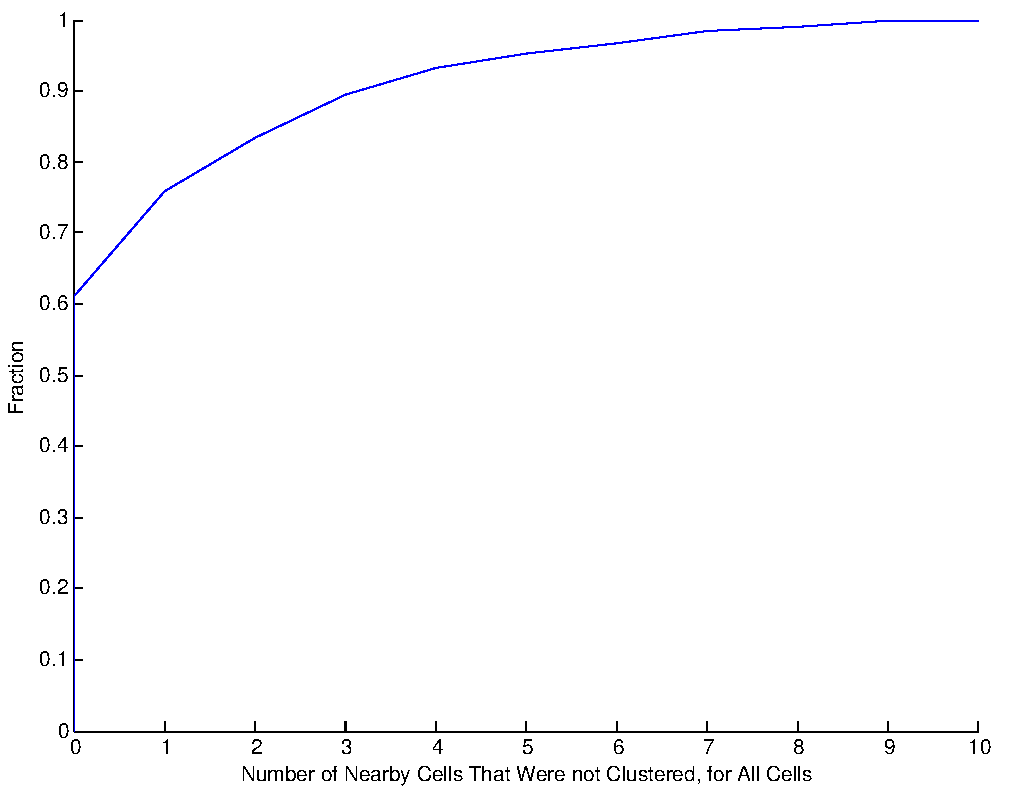
\includegraphics[width=\textwidth]{figs/cluster_incomp_cdf}
                \caption{The CDF of the cluster incompleteness under the same 
conditions. Approximately 90\% of the cells have less than 5 nearby 
unclustered neighbors.}
                \label{fig:cluster_incomp_cdf}
        \end{subfigure}
				\caption{Cluster incompleteness measurements.}
				\label{fig:cluster_incomp}
\end{figure*}
\subsection{Effectiveness of clustering algorithm}
\label{sec:effectiveness}
In this section we present the most important results of our project: an 
empirical validation of the clustering algorithm from the point of view of 
the efficiency of the clusters that it outputs.

We are only able to experimentally evaluate the quality of clusters in the 
MDC dataset, since it is the only one for which we have GPS information. We 
choose the MDC GPS logs as our source of location data for the cell towers 
for two reasons. First, as discussed in Section~\ref{sec:location_stats}, 
there are more cells in the MDC dataset covered by the GPS logs than by the 
open dataset. Second, because the GPS logs measure the \textit{user's} 
location when he or she was connected to that tower, it provides a 
semantically more accurate value -- after all, as discussed in
Section~\ref{sec:intro}, the ultimate goal of the clustering algorithm is to provide data 
that will be fed to an algorithm that predicts \textit{user's} movements.
\subsubsection{Metrics}



We define two metrics for assessing a cluster's quality: cluster distance and 
cluster incompleteness.

\paragraph{Cluster Distance} the average distance between cells in a cluster. 
A good algorithm will group together towers that are geographically close and 
therefore clusters will have a low distance. The cluster distance is measured 
in meters.

\paragraph{Cluster incompleteness} For a cell $k$, this is the number of 
cells within $\delta_{incomp}$ meters of it that are not in the same cluster 
as $k$. Intuitively this measures if there are potentially oscillating towers 
that are not being clustered together. We can think of the cluster 
incompleteness as the dual of the cluster distance: the former favors 
aggressive algorithms while the latter encourages conservative approaches. 
Another way to see the benefit of using two metrics is noting that there are 
trivial solutions that minimize distance or incompleteness (each cell in its 
own cluster and one huge cluster with all cels, respectively), but there are 
no trivial solutions that minimize both metrics at the same time. We use
$delta_{incomp} = 500$~meters.

\subsubsection{Cluster distance}

In order to provide some confidence in the precision of the results, we only 
consider cells that were seen more than once in the GPS logs, with a standard 
deviation less than 500 meters. Only clusters in which more tha 70\% of cells 
meet this criteria are analyzed. This meant that only 80 clusters, or 9.21\% 
of the total, could be analyzed. Although this is a small fraction, there is 
no reason to think it is a biased sample if we assume there is no correlation 
between GPS precision and clustering inefficiency. Therefore, the results 
should hold for the entirety of the clusters, and, we conjecture, for other 
datasets too.

Figure~\ref{fig:cluster_distance} show the histogram and CDF of the cluster 
distances. The results confirm that the algorithm is clustering towers that 
are largely close to each other: only one cluster (1.25\%) had a cluster 
distance greater than 500\,m.

\subsubsection{Cluster incompleteness}

The measurements for cluster incompleteness are presented in
Figure~\ref{fig:cluster_incomp}. The average incompleteness for all cells with GPS data 
is 0.52 (standard deviation 1.37). This is a surprisingly low value and 
indicates that the algorithm works well -- very few cells are not in the same 
cluster as their nearby neighbors.

\section{Conclusion}
\label{sec:conclusion}
We have evaluated a clustering algorithm used to eliminate the oscillation 
effect in cellular mobility prediction. Our main contribution is the use of 
GPS data to evaluate if the clustered towers are geographically close to each 
other, which would be circumstantial evidence in favor of the clustering 
algorithm. We find that the clustering algorithm proposed in \cite{
mobilityprofiler} performs well on the two metrics we define, cluster 
distance and cluster incompleteness.

As part of future work, we would like to repeat the experiments here with 
more data. As discussed before, only 9.44\% of the clusters in the MDC 
dataset had enough information to be reliably processed by the algorithm. One 
possible alternative is the professional cell tower location database 
provided by Navizon~\cite{navizon}. Another avenue of research is to 
investigate clustering algorithms that use a different clustering quality 
metric. One possible approach would be the modularity metric defined by 
Newman and Girvan~\cite{newman}. There is also a large body of literature on 
clustering in theoretical computer science, especially in social networks: 
Andersen and Peres find sparse cuts efficiently in~\cite{sparsecuts}, while 
Aroroa et. al try to find overlapping communities \cite{overlapping}. Finding 
overlapping communities has interesting applications for dealing with the 
oscillation effect, since towers can conceivably in more than one cluster.

\bibliographystyle{IEEEtranS}
\bibliography{eecs589Report}

\end{document}
